% !TeX root = ../main.tex

\chapter{系统测试}

\section{测试概要}
系统测试是系统开发过程中必不可少的重要阶段,是确保系统开发质量的关键,它贯穿于系统开发的整个过程,尽可能地发掘系统中存在的问题和错误,可以及时地进行纠错,促进系统开发工作高效有质量地进行.

\subsection{测试环境}
RISC-V指令集模拟器的测试环境分为软件模拟环境和硬件对照环境,软件模拟环境是系统设计使用到的第三方库和模拟器的宿主机环境,硬件对照环境主要是芯片开发过程中的FPGA开发板S2C Single U440平台以及流片后的真实芯片环境.具体的模拟器环境如表~\ref{tab:env}所示.
\begin{table}[h]
    \centering
    \caption{系统测试环境}
    \label{tab:env}
    \begin{tabular}{cc}
      \toprule
      名称	& 说明\\
      \midrule
    Ubuntu20.04	& \multicolumn{1}{c}{模拟器的宿主机环境}\\
    Qt5	& \multicolumn{1}{c}{Qt5的UI类库}\\
    BBL(berkele-bootloader)	& \multicolumn{1}{c}{RISC-V官方的bootloader}\\
    linux-v5.10    & \multicolumn{1}{c}{目标程序linux内核版本}\\
    busybox-1.32.1 & \multicolumn{1}{c}{linux命令集合}\\
      \bottomrule
    \end{tabular}
\end{table}


\subsection{概述}
本模拟器的测试采用测试驱动开发方式进行,主要过程如下:


(1) 根据需求分析中确定的芯片开发团队成员需求和系统概要设计中划分的四个功能模块,采用黑盒法设计对应的测试用例,当各个功能模块代码实现后立刻开始测试.


(2) 根据需求分析中的需求规格说明,使用场景法对模拟器进行配置项测试,测试模拟器的业务功能是否满足需求.


(3) 最后进行系统测试,重点测试linux内核移植过程中的MMU启动,挂载PLIC外设,以及调试功能是否满足后续的系统软件移植开发需求.


\section{测试分析}
测试分析主要对模拟器的测试需求进行分析,包含可以直接获取的显式功能性需求和系统中隐含的隐性需求比如模拟器运行速度.在系统开发的不同阶段,测试的需求也有所不同,本节所分析的测试需求有:模块测试需求,配置项测试需求和系统测试需求.下面对主要的测试需求展开分析.

\subsection{模块测试需求获取}
根据系统概要设计,本模拟器分为四个功能模块,下面对各个功能模块的测试需求进行分析:


(1) 预加载模块: 该模块解析模拟器启动参数,获取指令集配置,对相应的指令集模块进行注册,为后续的指令译码,以及功能函数调用提供所需的数据,依据概要设计的要求,主要测试该模块能否将所需指令集全部注册进解码器,并且在后续译码执行过程中调用正确的功能函数.


(2) CPU和总线模块: 该模块用于模拟处理器执行过程中的硬件行为,依据概要设计的要求,主要测试该模块的寄存器读写过程;访存请求涉及到的MMU行为,包括快表查询,iCache查询,通过页表的地址翻译过程;经过总线的mmio请求过程.主要测试其正确性.


(3) 中断控制器模块: 该模块用于模拟中断控制器的软硬件行为,依据概要设计的要求,主要测试通过PLIC挂载设备的中断请求过程能够被处理器响应,中断控制器能够做到规范文档的功能要求.

(3) 调试和UI模块: 该模块提供前端窗口交互功能和相应的调试功能,是本系统的重点测试部分,依据概要设计的要求,主要测试窗口对象和后端模拟器对象间的通信情况,包括断点信息的设置,处理器状态查询,调试模式下的UI更新情况等,既要测试其正确性,也要测试调试模式下的性能是否满足规范文档的要求.


\subsection{配置项测试需求获取}
根据RISC-V指令集模拟器的需求规格说明书,对于系统软件开发测试人员的需求进行配置项测试,主要是对模拟器加载目标程序的流程测试,以及后续目标程序的流程控制测试,包括设置断点,单步调试,寄存器/内存查询,外部中断信号发送.系统软件开发测试人员通过对目标程序的流程控制,可以方便地进行软件移植工作,加快系统软件的开发迭代.

\subsection{系统测试需求获取}
根据需求规格说明书,本模拟器需要进行系统软件的移植测试.包括了Bootload和Linux内核,在此移植过程中,对模拟器的整体功能部件进行测试,主要有Linux加载过程中的MMU启动,PLIC挂载外设,并将中断源通过设备注册到操作系统.

\section{测试用例设计}
针对系统开发的各个阶段,测试用例的设计和采用的设计方法都有所不同,下面对各个阶段的测试用例进行设计.

\subsection{模块测试用例设计}
依据模块测试的需求,对RISC-V指令集模拟器的四个功能模块进行测试, 各个模块的测试用例设计如下:


(1) 预加载模块: 根据测试需求,该模块的功能是根据模拟器启动参数加载对应的指令集模块,对指令列表进行注册,将指令格式和对应的功能函数绑定起来,完成解码器的初始化工作,该模块检测到未定义指令模块,会发出告警信息,提示未定义行为.具体的测试用例设计如表~\ref{tab:test1}所示.
\begin{table}[h]
    \centering
    \caption{指令集模块测试用例表}
    \label{tab:test1}
    \begin{tabular}{clll}
      \toprule
      \multicolumn{1}{c}{序号} & \multicolumn{1}{c}{输入} & \multicolumn{1}{c}{预期输出} &\multicolumn{1}{c}{说明}\\
      \midrule
  1	& \multicolumn{1}{m{3.5cm}}{指令集标准拓展rv64imafdc} & \multicolumn{1}{m{3.5cm}}{模拟器注册指令列表的全部内容,解码器保存指令格式和功能函数的映射} & \multicolumn{1}{m{3.5cm}}{验证功能模块的有效性}\\
  \hline
  2	& \multicolumn{1}{m{3.5cm}}{未定义指令集拓展rv64jkl} & \multicolumn{1}{m{3.5cm}}{提示未定义的指令集拓展} & \multicolumn{1}{m{3.5cm}}{验证功能模块的健壮性}\\
  \hline
  3	& \multicolumn{1}{m{3.5cm}}{未定义功能函数的自定义指令} & \multicolumn{1}{m{3.5cm}}{解码器提示功能函数未定义} & \multicolumn{1}{m{3.5cm}}{验证功能模块的健壮性}\\
      \bottomrule
    \end{tabular}
\end{table}


(2) CPU和总线模块: 根据测试需求,该模块的功能是模拟指令执行过程中的硬件行为,包括寄存器,MMU,缓存,内存,IO控制器等,测试目的是验证该模块的硬件行为模拟和真实硬件行为一致.该模块的输入总是已注册的指令,不会有其他未定义输入,主要检测是否达到预期输出,具体的测试用例设计如表~\ref{tab:test2}所示.
\begin{table}[h]
    \centering
    \caption{CPU和总线测试用例表}
    \label{tab:test2}
    \begin{tabular}{clll}
      \toprule
      \multicolumn{1}{c}{序号} & \multicolumn{1}{c}{输入} & \multicolumn{1}{c}{预期输出} &\multicolumn{1}{c}{说明}\\
      \midrule
  4	& \multicolumn{1}{m{3.5cm}}{汇编指令ld t0 1000} & \multicolumn{1}{m{3.5cm}}{通用数据寄存器t0内容0x1000} & \multicolumn{1}{m{3.5cm}}{验证功能模块的有效性}\\
  \hline
  5	& \multicolumn{1}{m{3.5cm}}{汇编指令csrw mtevc, t0} & \multicolumn{1}{m{3.5cm}}{CSR寄存器mtevc被写入t0寄存器的值} & \multicolumn{1}{m{3.5cm}}{验证功能模块的有效性}\\
  \hline
  6	& \multicolumn{1}{m{3.5cm}}{机器模式下的内存查询请求} & \multicolumn{1}{m{3.5cm}}{MMU显示Mbare模式,不进行地址翻译} & \multicolumn{1}{m{3.5cm}}{验证功能模块的有效性}\\
  \hline
  7	& \multicolumn{1}{m{3.5cm}}{监管模式下的sv39内存查询请求} & \multicolumn{1}{m{3.5cm}}{MMU查询页表,输出地址翻译过程} & \multicolumn{1}{m{3.5cm}}{验证功能模块的有效性}\\
  \hline
  8	& \multicolumn{1}{m{3.5cm}}{和序号7同一地址的监管模式下的sv39内存查询请求} & \multicolumn{1}{m{3.5cm}}{MMU查询快表,TLB命中,输出查询内容} & \multicolumn{1}{m{3.5cm}}{验证功能模块的有效性}\\
      \bottomrule
    \end{tabular}
\end{table}

(3) 中断控制器模块: 根据测试需求,该模块的功能是将内存映射的I/O设备挂载到中断控制器,和处理器进行通信.测试目的为了验证中断控制器能够对外部中断信号源进行有效裁决,并配合处理器完成外部中断的流程,以及测试当外部中断源优先级低于处理器门限寄存器时能否屏蔽该中断源.具体的测试用例设计如表~\ref{tab:test3}所示.
\begin{table}[h]
    \centering
    \caption{中断控制器测试用例表}
    \label{tab:test3}
    \begin{tabular}{clll}
      \toprule
      \multicolumn{1}{c}{序号} & \multicolumn{1}{c}{输入} & \multicolumn{1}{c}{预期输出} &\multicolumn{1}{c}{说明}\\
      \midrule
  9	& \multicolumn{1}{m{3.5cm}}{对UART的mmio请求} & \multicolumn{1}{m{3.5cm}}{前端窗口输出请求回复内容} & \multicolumn{1}{m{3.5cm}}{验证功能模块的有效性}\\
  \hline
  10	& \multicolumn{1}{m{3.5cm}}{UART以优先级2挂载到PLIC,处理器机器模式和监管模式的门限优先级设置为3} & \multicolumn{1}{m{3.5cm}}{处理器不再响应UART中断源的外部中断请求} & \multicolumn{1}{m{3.5cm}}{验证功能模块的健壮性}\\
  \bottomrule
    \end{tabular}
\end{table}


(4) 调试模块和UI: 根据测试需求,该模块的功能是对目标程序运行流程进行控制,切换至调试模式进行断点设置,寄存器/内存查询,单步调试等功能,测试目的是验证该模块通过UI将调试信号发送给后端模拟器,并进行断点匹配的过程,还有验证寄存器/内存查询的正确性,以及查询无效内存地址给出告警信息的过程.具体测试用例设计如表~\ref{tab:test4}所示.
\begin{table}[h]
    \centering
    \caption{调试模块和UI测试用例表}
    \label{tab:test4}
    \begin{tabular}{clll}
      \toprule
      \multicolumn{1}{c}{序号} & \multicolumn{1}{c}{输入} & \multicolumn{1}{c}{预期输出} &\multicolumn{1}{c}{说明}\\
      \midrule
  11	& \multicolumn{1}{m{3cm}}{调试模式下单步执行信号} & \multicolumn{1}{m{4cm}}{模拟器执行完一条指令后发出更新信号,前端UI刷新寄存器状态} & \multicolumn{1}{m{3.5cm}}{验证功能模块的有效性}\\
  \hline
  12	& \multicolumn{1}{m{3cm}}{断点信息pc core0 0x80000000} & \multicolumn{1}{m{4cm}}{核0在PC=0x80000000处匹配断点,进入调试模式,输出断点信息} & \multicolumn{1}{m{3.5cm}}{验证功能模块的有效性}\\
  \hline
  13	& \multicolumn{1}{m{3cm}}{内存地址0x80000000查询信号} & \makecell[l]{0xif80006f\\
  对应汇编指令j pc+504\\
  表示跳转到reset\_vector
  } & \multicolumn{1}{m{3.5cm}}{验证功能模块的有效性}\\
  \hline
  14	& \multicolumn{1}{m{3cm}}{内存地址0xffffffff查询信号} & \multicolumn{1}{m{4cm}}{发出警告信息,无效内存地址} & \multicolumn{1}{m{3.5cm}}{验证功能模块的健壮性}\\
      \bottomrule
    \end{tabular}
\end{table}

\subsection{配置项测试用例设计}
依据配置项测试需求,采用基于实际业务的场景设计法对RISC-V指令集模拟器的RISC-V架构目标程序调试功能进行测试用例设计.该功能设计的基本流有:1.设置断点信息,点击应用后,调试窗口发送断点信号到模拟器后端,添加新的断点信息到处理器断点检测列表; 2.删除处理器断点检测列表中的某一项; 3.点击单步执行,模拟器进行一次取值,译码,执行周期,更新寄存器状态窗口,输出当前指令到指令历史窗口; 4.输入待查询内存地址,点击查询,模拟器进入MMU访存逻辑,查询当前地址内容; 5.点击运行,模拟器进入运行模式,将交互信息输出到交互窗口; 该功能的备选流有: 1.设置断点信息错误,导致处理器断点检测列表添加失败; 2.输入无效地址导致内存查询失败,发出告警信息.基本流和备选流可以组合成各个场景,进而对每个场景设计测试用例,具体的测试用例设计如表~\ref{tab:test5}所示.
\begin{table}[h]
    \centering
    \caption{配置型测试用例表}
    \label{tab:test5}
    \begin{tabular}{clll}
      \toprule
      \multicolumn{1}{c}{序号} & \multicolumn{1}{c}{操作} & \multicolumn{1}{c}{预期输出} &\multicolumn{1}{c}{说明}\\
      \midrule
  15	& \multicolumn{1}{m{3.5cm}}{设置断点信息,点击应用} & \multicolumn{1}{m{3.5cm}}{处理器断点检测列表添加成功} & \multicolumn{1}{m{3.5cm}}{基本流1,备选流1}\\
  \hline
  16	& \multicolumn{1}{m{3.5cm}}{删除某一断断点信息} & \multicolumn{1}{m{3.5cm}}{删除成功} & \multicolumn{1}{m{3.5cm}}{基本流2}\\
  \hline
  17	& \multicolumn{1}{m{3.5cm}}{点击单步执行} & \multicolumn{1}{m{3.5cm}}{寄存器状态更新,指令历史窗口更新} & \multicolumn{1}{m{3.5cm}}{基本流3}\\
  \hline
  18	& \multicolumn{1}{m{3.5cm}}{输入内存地址,点击查询} & \multicolumn{1}{m{3.5cm}}{对应内存地址的内容} & \multicolumn{1}{m{3.5cm}}{基本流4,备选流2}\\
  \hline
  19	& \multicolumn{1}{m{3.5cm}}{调试模式下点击运行} & \multicolumn{1}{m{3.5cm}}{更新目标程序的交互信息} & \multicolumn{1}{m{3.5cm}}{基本流5}\\
      \bottomrule
    \end{tabular}
\end{table}


\subsection{系统测试用例设计}
依据系统测试需求,主要对RISC-V指令集模拟器进行稳定性测试,容错性测试和性能测试,下面分别对各个测试进行测试用例设计:


(1)	稳定性测试: 依据系统测试需求,模拟器需要在加载给定的目标程序后不间断地稳定运行.因此稳定性测试设计为模拟器加载linux内核运行top程序三天,预期结果是模拟器可以一直持续运行,并且实时检测模拟CPU的进程状态.


(2)	容错性测试: 依据系统测试需求,从一下两个方面进行测试用例设计: 加载含有未定义指令的程序,检测程序能否陷入对应的异常(illegal instruction);设置错误的断点信息,检测模拟器在端点检测逻辑是否会发生因设计错误导致的程序崩溃.


(3)	性能测试: 依据系统测试需求,记录模拟器在断点检测列表为空的状态下,和含有断点检测列表的状态下的MIPS(Million instruction per-second),和实际的硬件MIPS做对比,测试模拟器模拟速度.另外从模拟器进行系统软件调试的功能考虑,记录了在模拟器和真在实硬件平台上的调试周期,进行对照测试,分析模拟器在软件移植/开发/测试流程中的性能.

\section{测试结果及分析}
使用各个测试阶段所设计的测试用例,对RISC-V指令集模拟器展开了单元测试,配置项测试和系统测试,具体测试结果如下:


(1) 在单元测试中对模拟器的四个功能模块都进行了测试,经过五次回归实验后,各个功能模块实际输出与预期输出达成一致,各个模块的功能和健壮性都得到了验证,达到了需求规格说明书中的需求。


(2) 在配置项测试中对模拟器的目标程序调试功能进行测试,各个测试用例的实际输出与预期输出一致,所测业务功能满足设计需求。


(3) 在系统测试中对模拟器进行稳定性测试、容错性测试和性能测试.稳定性测试时系统正常运行情况如图~\ref{fig:run}所示;容错性测试达到了预测的结果.从测试结果可以看出吸烟检测系统的可靠性满足需求规格说明书中的需求;通过和真实硬件平台的对照,在系统软件移植开发流程中,模拟器的软件迭代周期要明显比硬件平台效率更高,性能要求也达到了预期的结果. 
\begin{figure}[h]
  \centering
  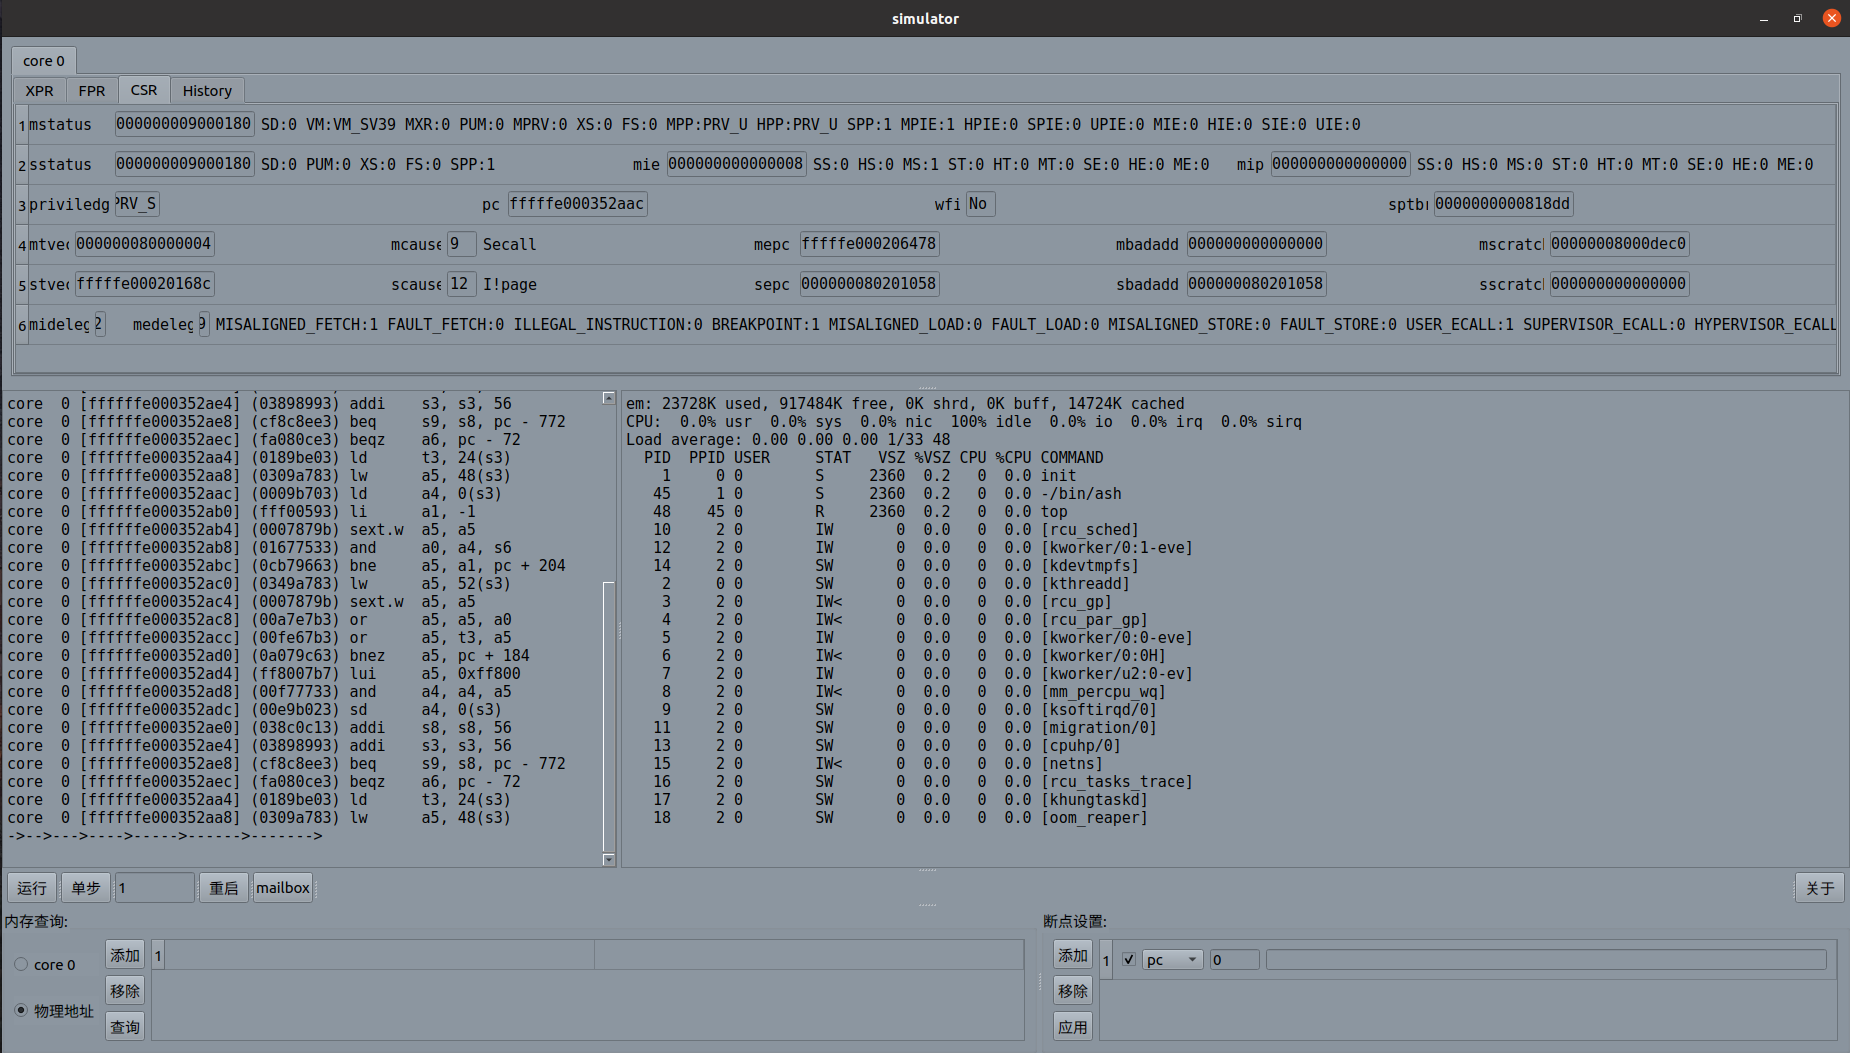
\includegraphics[width=1.0\textwidth]{run.png}
  \caption{模拟器正常运行UI界面}
  \label{fig:run}
\end{figure}

通过比对模拟器和FPGA硬件平台的软件开发周期,可以看出RISC-V指令集模拟器带来的明显效率提升。如表~\ref{tab:cmp}.
\begin{table}[h]
  \centering
  \caption{模拟器和硬件平台对照表}
  \label{tab:cmp}
  \renewcommand\arraystretch{1.1}
  \begin{tabular}{cccc}
    \toprule
    \multicolumn{1}{c}{软件调试流程} & \multicolumn{1}{l}{模拟器平台} & \multicolumn{1}{l}{FPGA平台} &\multicolumn{1}{l}{流片的S2C平台}\\
    \midrule
目标程序交叉编译	& \multicolumn{1}{m{3cm}}{<1min} & \multicolumn{1}{m{3cm}}{<1min} & \multicolumn{1}{m{3cm}}{<1min}\\
\hline
粘贴fsbl	& \multicolumn{1}{m{3cm}}{-} & \multicolumn{1}{m{3cm}}{-} & \multicolumn{1}{m{3cm}}{5min}\\
\hline
vivado平台烧录	& \multicolumn{1}{m{3cm}}{-} & \multicolumn{1}{m{3cm}}{10min} & \multicolumn{1}{m{3cm}}{-}\\
\hline
flash烧录	& \multicolumn{1}{m{3cm}}{-} & \multicolumn{1}{m{3cm}}{-} & \multicolumn{1}{m{3cm}}{10min}\\
\hline
启动程序	& \multicolumn{1}{m{3cm}}{<1min} & \multicolumn{1}{m{3cm}}{5min} & \multicolumn{1}{m{3cm}}{5min}\\
\hline
调试手段	& \multicolumn{1}{m{3cm}}{断点/单步/查询} & \multicolumn{1}{m{3cm}}{Jtag单步} & \multicolumn{1}{m{3cm}}{硬件波形}\\
    \bottomrule
  \end{tabular}
\end{table}


\section{测试结论}
经过一系列的测试,RISC-V指令集模拟器能够长时间稳定运行,进行目标程序的跨平台模拟执行.对于可能的异常行为,模拟器提供了丰富的调试手段,方便芯片开发团队进行问题排查,针对发现的硬件缺陷或者软件错误,及时进行修正,进行下一轮的测试迭代.一方面可以对硅后处理器验证起到辅助验证的作用,一方面也能够加快系统软件的开发速度,脱离硬件进行并行的移植开发工作,大大缩短了系统软件的开发周期.


但是在实际的使用过程中,本模拟器对于后续的驱动程序开发,需要经常对各种外设进行模拟,这部分的模拟主要参照各个设备厂商IP,对于模拟过程可能产生的错误较难及时发现.此外在芯片开发过程中,需要及时对模拟器进行迭代,修正与真实芯片的功能差异,这就需要软件开发人员和硬件设计人员及时有效地沟通,无法做到职责分离.因此本模拟器还是存在较大的改进空间.